\documentclass[8pt]{article}

\usepackage{amsmath, amssymb, amsfonts}
\usepackage{graphicx}

\usepackage{hyperref}
\usepackage[margin=1in]{geometry}
\usepackage{fancyhdr}
\usepackage{parskip}
\usepackage{titlesec}
\usepackage{setspace}

\title{CAB320 - Artificial Intelligence Study Notes}
\author{Jaden Ussher}
\date{Last modified on 2022/03/02}

% Custom header and footer
\pagestyle{fancy}
\fancyhf{}
\fancyhead[L]{CAB320 Artificial Intelligence}
\fancyhead[R]{Study Notes}
\fancyfoot[C]{\thepage}

% Title formatting
\titleformat{\section}{\large\bfseries}{\thesection}{1em}{}
\titleformat{\subsection}{\normalsize\bfseries}{\thesubsection}{1em}{}
\titleformat{\subsubsection}{\normalsize\itshape}{\thesubsubsection}{1em}{}

% Adjust line spacing
\singlespacing

\begin{document}

\maketitle
\small
\newpage

\tableofcontents

\newpage
\section{Week 2 - Discrete Math Tools}
\subsection{Key Discrete Math Concepts for AI}
\begin{itemize}
    \item Recurrence relations and recursive functions
    \item Graphs and trees
    \begin{itemize}
        \item Data structure, abstraction, object-oriented programming
    \end{itemize}
    \item Graph properties
    \begin{itemize}
        \item Directedness, paths, connectivity, connected components, cycles, roots, sinks
    \end{itemize}
    \item Dijkstra's algorithm
    \begin{itemize}
        \item Computation of the shortest paths from a source to all other vertices
    \end{itemize}
\end{itemize}

\subsection{Graphs and Their Importance in AI}
\begin{figure}[h]
    \centering
    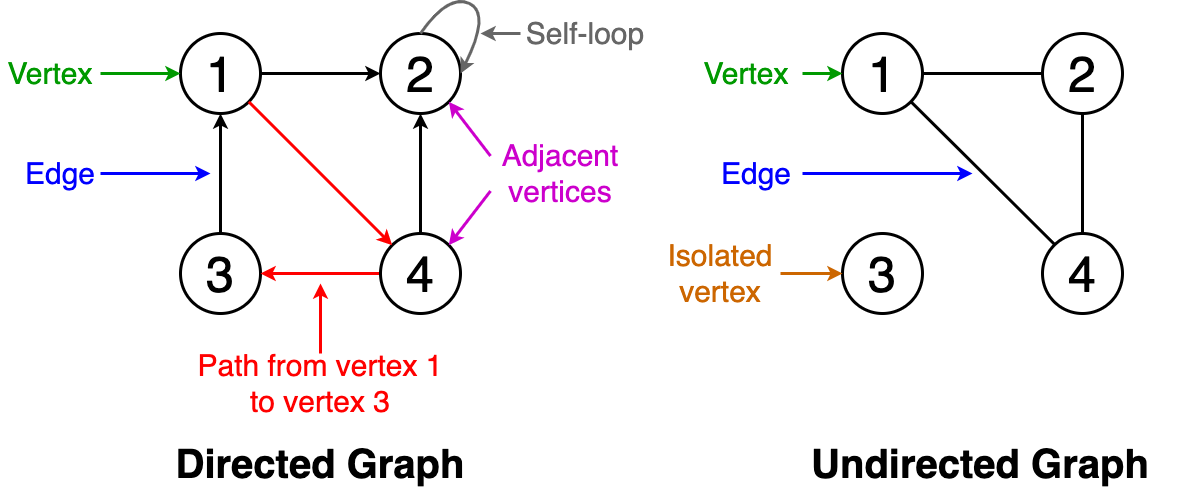
\includegraphics[width=0.5\linewidth]{images/1_xpy7aax3dIU12HVrGd_siQ.png}
    \caption{Graph Basics}
    \label{fig:enter-label}
\end{figure}

\begin{itemize}
    \item A graph \( G \) is a pair \( (V, E) \) where \( V \) is a set of vertices and \( E \) is a set of pairs of vertices called edges.
    \item Graphs do not need a visual representation to exist.
    \item Directed graphs (digraphs) have ordered edges, called arcs.
    \item Vertices are also known as nodes.
    \item In AI, graphs are used for:
    \begin{itemize}
        \item Planning problems: Finding a “good” sequence of actions can be reduced to finding a “good” path in an associated state graph.
        \item Knowledge representation: Social networks, scene representation, protein folding, etc.
    \end{itemize}
\end{itemize}

\subsection*{Graph Representations}
\subsubsection*{Adjacency Matrix}
\begin{itemize}
    \item For undirected graphs: A symmetric matrix where \( A[i][j] = 1 \) if there is an edge between vertices \( i \) and \( j \), otherwise \( 0 \).
    \item For directed graphs: \( A[i][j] = 1 \) if there is an arc from \( i \) to \( j \).
\end{itemize}

\subsubsection*{Vertex-Arc Incidence Matrix}
\begin{itemize}
    \item Represents the incidence of vertices and arcs.
\end{itemize}

\subsubsection*{Adjacency List}
\begin{itemize}
    \item Use dictionaries in Python where keys are vertices and values are lists of neighbors.
    \item Efficient for sparse graphs.
\end{itemize}

\subsection*{Graph Properties}
\begin{itemize}
    \item Directedness: Graphs can be directed or undirected.
    \item Paths and connectivity:
    \begin{itemize}
        \item A path is a sequence of vertices connected by edges.
        \item Connectivity determines if there is a path between every pair of vertices.
        \item A connected component is a maximal connected subgraph.
    \end{itemize}
    \item Cycles: A path that starts and ends at the same vertex without repeating any edge or vertex.
    \item In-degree and Out-degree:
    \begin{itemize}
        \item In-degree: Number of incoming arcs to a vertex.
        \item Out-degree: Number of outgoing arcs from a vertex.
    \end{itemize}
\end{itemize}

\subsection*{Special Graphs}
\subsubsection*{Clique}
\begin{itemize}
    \item A clique is a subset of vertices such that every two distinct vertices are adjacent.
    \item Maximal clique: A clique that cannot be extended by including one more adjacent vertex.
\end{itemize}

\subsubsection*{Interval Graph}
\begin{itemize}
    \item Vertices represent intervals, and there is an edge between two vertices if their corresponding intervals intersect.
    \item Always contains a vertex whose neighbors form a clique.
\end{itemize}

\subsection*{Trees}
\begin{itemize}
    \item A tree is a connected, acyclic undirected graph. Equivalent conditions for trees:
    \begin{itemize}
        \item Connected and acyclic.
        \item Adding any edge creates a cycle.
        \item Removing any edge disconnects the graph.
        \item Unique simple path between any two vertices.
    \end{itemize}
\end{itemize}
\newpage
\subsection{Dijkstra's Algorithm}
\begin{itemize}
    \item Purpose: Find shortest paths from a source vertex to all other vertices in a weighted graph.
    \item Method:
    \begin{itemize}
        \item Initialize distances from the source to all vertices as infinity except the source itself, which is zero.
        \item Use a priority queue to repeatedly extract the vertex with the minimum distance.
        \item Update the distances of the adjacent vertices.
    \end{itemize}
\end{itemize}

\subsubsection*{Example 1}
\begin{figure}[h]
    \centering
    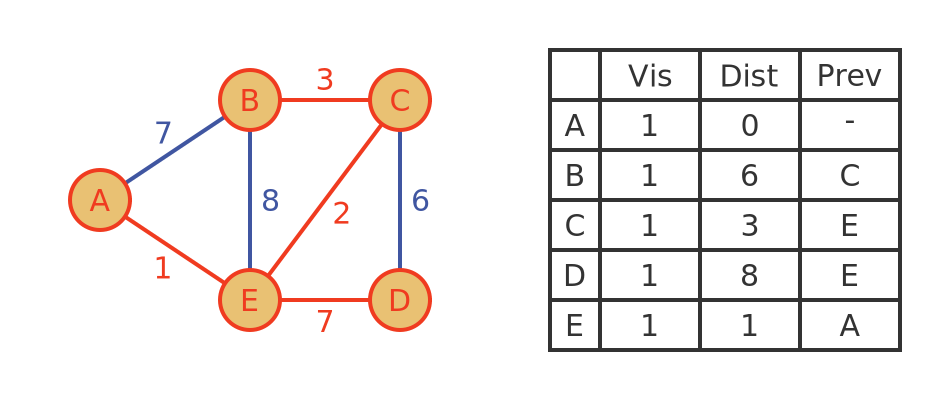
\includegraphics[width=0.5\linewidth]{images/algorithm-5.png}
    \caption{Dijkstra's Algorithm Visual Example}
    \label{fig:enter-label}
\end{figure}


\subsubsection*{Example 2}

\begin{verbatim}
Graph: (V, E) with weights
    V = {A, B, C, D}
    E = {(A, B, 1), (A, C, 4), (B, C, 2), (B, D, 5), (C, D, 1)}
Steps:
1. Initialize distances: dist[A]=0, dist[B]=∞, dist[C]=∞, dist[D]=∞
2. Extract A: dist[A]=0
    Update dist[B]=1, dist[C]=4
3. Extract B: dist[B]=1
    Update dist[C]=3, dist[D]=6
4. Extract C: dist[C]=3
    Update dist[D]=4
5. Extract D: dist[D]=4
Result: Shortest paths from A
    A -> B -> C -> D with distances 0, 1, 3, 4 respectively.
\end{verbatim}

\subsection*{Correctness of Dijkstra's Algorithm}
\begin{itemize}
    \item \textbf{Invariant Hypothesis}:
    \begin{itemize}
        \item For each vertex \( v \), \( \text{dist}[v] \) is an upper bound of the cost of a cheapest path from the source to \( v \).
        \item If \( v \) has been removed from the priority queue, \( \text{dist}[v] \) is the cost of the cheapest path.
    \end{itemize}
    \item Proof by induction on the size of \( V - L \) (where \( L \) is the set of unfinalized vertices).
    \item \textbf{Lemma}: If \( T \) is the tree of finalized vertices, any non-finalized vertex \( a \) adjacent to \( T \) has the cheapest path via its parent.
    \item \textbf{Contradiction}:
    \begin{itemize}
        \item If there is a strictly cheaper path, it would imply incorrect extraction order, violating the algorithm's logic.
    \end{itemize}
\end{itemize}

\section{Week 3 - Intelligence Agents \& Uniformed Search}
\subsection{Intelligence Agents}
\subsection{Key Concepts}
\subsubsection*{Agents and Environments}
\begin{itemize}
    \item Agents include humans, robots, softbots, thermostats, etc.
    \item The agent function maps from percept histories to actions.
    \item Agents interact with environments through sensors and actuators.
\end{itemize}

\subsubsection*{Vacuum-Cleaner World}
\begin{itemize}
    \item Percepts: Location and contents, e.g., [A, Dirty].
    \item Actions: Left, Right, Suck, NoOp.
    \item Example: A vacuum-cleaner agent must decide its actions based on its current percept.
\end{itemize}

\subsubsection*{Rationality}
\begin{itemize}
    \item A rational agent chooses any action that maximizes the expected value of the performance measure given the percept sequence to date.
    \item Rationality maximizes expected outcome while perfection maximizes actual outcome.
    \item Rational does not mean omniscient or perfect.
\end{itemize}

\subsubsection*{P.E.A.S. Framework}
\begin{itemize}
    \item To design a rational agent, we must specify the task environment, which consists of:
    \begin{itemize}
        \item Performance measure
        \item Environment
        \item Actuators
        \item Sensors
    \end{itemize}
    \item Examples:
    \begin{itemize}
        \item Automated taxi: Safety, streets, steering, video.
        \item Internet shopping agent: Price, WWW sites, display, HTML pages.
        \item Part-picking robot: Percentage of parts in correct bins, conveyor belt, jointed arm, camera.
    \end{itemize}
\end{itemize}

\subsubsection*{Environment Types}
\begin{itemize}
    \item Deterministic vs. stochastic: Is the next state perfectly predictable?
    \item Static vs. dynamic: Does the environment change while the agent deliberates?
    \item Fully vs. partially observable: Does the agent have access to all relevant information?
    \item Single-agent vs. multi-agent: Are there other agents in the environment?
    \item Known vs. unknown: Does the agent understand the laws governing the environment?
    \item Episodic vs. sequential: Are past actions relevant to the current decision?
    \item Discrete vs. continuous: Are states and time intervals fixed or continuous?
\end{itemize}

\subsubsection*{Agent Types}
\begin{itemize}
    \item Simple reflex agents: Choose actions based on current percept.
    \item Reflex agents with state: Have memory or a model of the world’s current state.
    \item Goal-based agents: Act to achieve specific goals.
    \item Utility-based agents: Maximize a utility function to measure performance.
    \item Learning agents: Improve their performance over time.
\end{itemize}

\subsubsection*{Examples of Agent Types}
\begin{itemize}
    \item Reflex Agents: Edge following robot.
    \item Model-Based Reflex Agent: Vacuum robot that counts the number of cells cleaned.
    \item Model-Based Goal-Based Agent: Sokoban agent.
    \item Model-Based Utility-Based Agent: Pacman player.
    \item General Learning Agent: Self-balancing robot.
\end{itemize}

\newpage
\subsection{Uniformed Search}
\subsubsection*{Planning Agents}
\begin{itemize}
    \item Planning agents ask "what if" and make decisions based on hypothesized consequences of actions.
    \item They must have a model of how the world evolves in response to actions.
    \item Formulation of a goal and consideration of how the world would be is essential.
    \item Distinguish between optimal vs. complete planning and planning vs. re-planning.
\end{itemize}

\subsection*{State Types}
Different types of states in planning and search problems are considered.

\subsection*{Search Problems}
A search problem consists of:
\begin{itemize}
    \item A state space.
    \item A successor function (with actions and costs).
    \item A start state and a goal test.
\end{itemize}
A solution is a sequence of actions (a plan) that transforms the start state to a goal state.

\subsection*{Example Problems}
\begin{itemize}
    \item Romania: Finding paths between cities.
    \item Vacuum world: A simple robotic agent cleaning a room.
    \item The 8-puzzle: Sliding puzzle game.
    \item The 8-queens problem: Placing 8 queens on a chessboard without threatening each other.
    \item Robotic assembly: Planning the sequence of actions for assembling parts.
\end{itemize}

\subsection{Tree Search Algorithms}
Tree search algorithms explore possible sequences of actions to find a solution.

\subsection{Uninformed Search Strategies}
Uninformed search strategies are methods that search the state space without any domain-specific knowledge. These include:
\begin{itemize}
    \item Breadth-First Search (BFS)
    \item Uniform-Cost Search
    \item Depth-First Search (DFS)
    \item Depth-Limited Search
    \item Iterative Deepening Search
\end{itemize}

\newpage
\subsubsection{Breadth-First Search (BFS)}
\begin{itemize}
    \item Explores all nodes at the present depth level before moving on to nodes at the next depth level.
    \item Initial frontier: \{A\}
    \item Frontier after expanding A: \{B, C\}
    \item Frontier after expanding B: \{C, D, E\}
    \item Frontier after expanding C: \{D, E, F, G\}
\end{itemize}
Properties: Complete and optimal for unweighted graphs, but has high memory requirements.

\begin{figure}[!h]
    \centering
    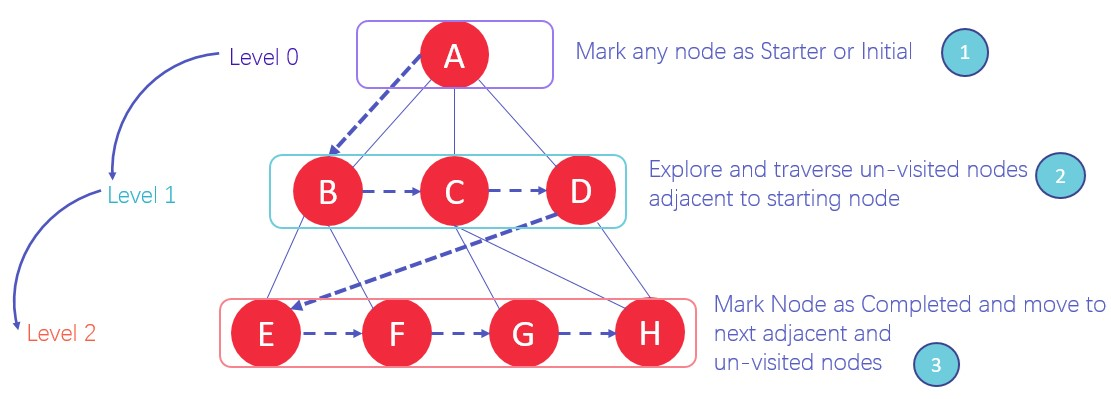
\includegraphics[width=0.5\linewidth]{images/020820_0543_BreadthFirs1ropped.jpg}
    \caption{BFS Algorithm}
    \label{fig:enter-label}
\end{figure}

\subsubsection{Uniform-Cost Search}
\begin{itemize}
    \item Expands the least-cost unexpanded node.
    \item Similar to Dijkstra's algorithm for shortest paths.
\end{itemize}

\begin{figure}[!h]
    \centering
    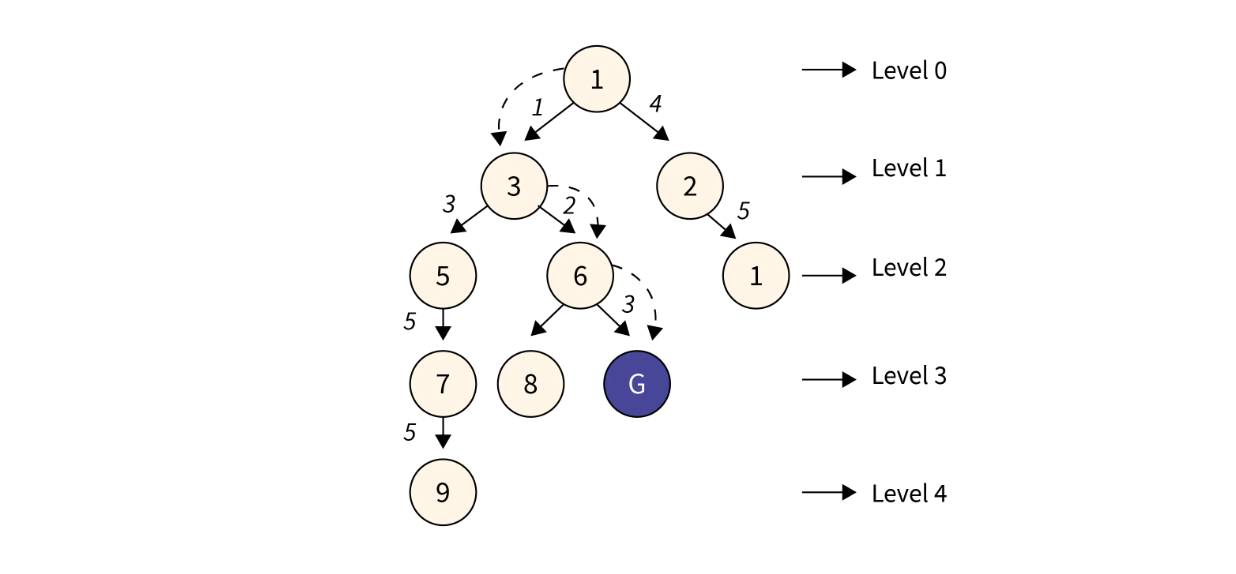
\includegraphics[width=0.5\linewidth]{images/uniform search.PNG}
    \caption{Uniform Cost Search Algorithm}
    \label{fig:enter-label}
\end{figure}

\subsubsection{Depth-First Search (DFS)}
\begin{itemize}
    \item Explores as far as possible along each branch before backtracking.
    \item Initial frontier: \{A\}
    \item Frontier after expanding A: \{B, C\}
    \item Frontier after expanding C: \{B, F, G\}
    \item Frontier after expanding G: \{B, F, N, O\}
\end{itemize}
Properties: May get stuck in infinite loops, not guaranteed to find the shortest path.

\begin{figure}[!h]
    \centering
    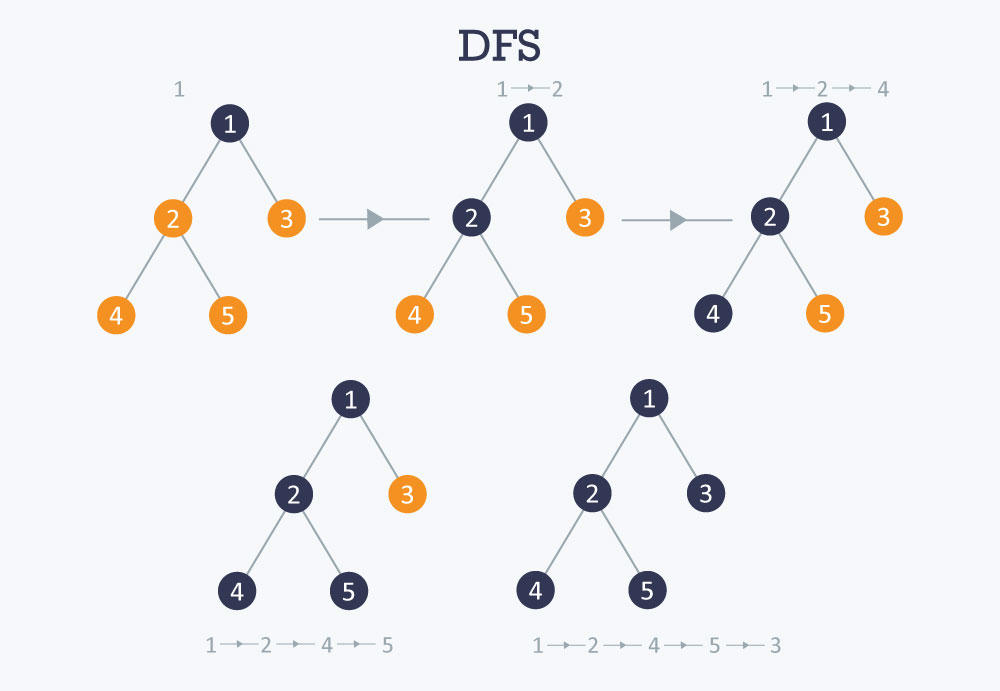
\includegraphics[width=0.5\linewidth]{images/DFS.jpg}
    \caption{Depth First Search Algorithm}
    \label{fig:enter-label}
\end{figure}

\newpage
\subsubsection{Depth-Limited Search}
\begin{itemize}
    \item Depth-first search with a limit on the depth.
    \item Useful for infinite depth or large search spaces.
\end{itemize}

\begin{figure}[!h]
    \centering
    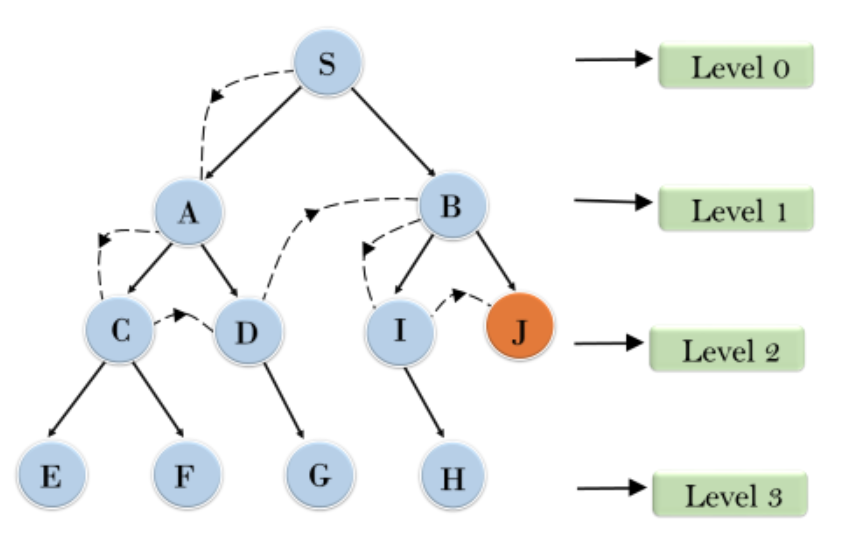
\includegraphics[width=0.5\linewidth]{images/dls.PNG}
    \caption{Depth Limited Search}
    \label{fig:enter-label}
\end{figure}

\subsubsection{Iterative Deepening Search}
\begin{itemize}
    \item Combines the benefits of BFS and DFS.
    \item Repeatedly applies DFS with increasing depth limits.
    \item Level 0: \{A\}
    \item Level 1: \{B, C\}
    \item Level 2: \{D, E, F, G\}
\end{itemize}
Properties: Complete and optimal like BFS, but with lower memory requirements.
\newpage
\subsection*{Implementation Considerations}
\subsection*{States vs. Nodes}
\begin{itemize}
    \item States represent physical configurations.
    \item Nodes represent states with additional information, such as parent nodes, actions, and path costs.
\end{itemize}

\subsubsection*{General Tree Search Algorithm}
The general tree search algorithm explores nodes in a tree structure, using different strategies to manage the frontier.

\subsubsection*{Search Strategies}
Different strategies impact the efficiency and effectiveness of finding a solution.

\subsubsection*{Graph Search}
\begin{itemize}
    \item Avoids expanding the same state multiple times.
    \item Maintains a frontier to explore and a set of explored nodes.
\end{itemize}
Example: Uniform-cost search on a subgraph of the Romania map.

\subsubsection*{Bidirectional Search}
\begin{itemize}
    \item Searches from both the start and goal states simultaneously.
    \item Can significantly reduce search time.
\end{itemize}

\newpage
\section{Wek 4 - A* Tree Search and Search Heuristics}
\subsection{A* Search Algorithm}
\begin{itemize}
    \item Combines the strengths of Uniform Cost Search (UCS) and Greedy Search.
    \item Uses both path cost \(g(n)\) and heuristic cost \(h(n)\).
    \item Expands nodes based on the evaluation function \(f(n) = g(n) + h(n)\).
\end{itemize}

\subsubsection*{Key Properties of A*}
\begin{itemize}
    \item \textbf{Completeness:} A* is complete if the branching factor is finite and the cost of every step is greater than a positive constant.
    \item \textbf{Optimality:} A* is optimal if the heuristic used is admissible (i.e., it never overestimates the true cost).
    \item \textbf{Admissible Heuristics:} Heuristic \(h(n)\) is admissible if \(0 \leq h(n) \leq h^*(n)\), where \(h^*(n)\) is the true cost to reach the goal from node \(n\).
    \item \textbf{Efficiency:} The efficiency of A* depends on the quality of the heuristic function. Better heuristics result in fewer nodes being expanded.
\end{itemize}

\subsubsection*{Example: A* Search for Pathfinding}
\begin{itemize}
    \item Consider finding a path in a grid from a start node \(S\) to a goal node \(G\).
    \item \textbf{Path Cost \(g(n)\):} The cost to reach node \(n\) from the start node \(S\).
    \item \textbf{Heuristic Cost \(h(n)\):} An estimate of the cost to reach the goal node \(G\) from node \(n\). For instance, Manhattan distance or Euclidean distance.
    \item \textbf{Evaluation Function \(f(n)\):} \(f(n) = g(n) + h(n)\).
    \item A* search explores nodes in order of increasing \(f(n)\) values.
\end{itemize}

\subsubsection*{Algorithm Steps}
\begin{enumerate}
    \item Initialize the open list with the start node \(S\).
    \item Initialize the closed list as empty.
    \item Loop until the open list is empty or the goal node is found:
    \begin{enumerate}
        \item Remove the node \(n\) with the lowest \(f(n)\) from the open list.
        \item If \(n\) is the goal node \(G\), reconstruct the path from \(S\) to \(G\).
        \item Generate successors of node \(n\).
        \item For each successor:
        \begin{itemize}
            \item Calculate \(g(\text{successor})\) and \(f(\text{successor})\).
            \item If the successor is not in the open list or has a lower \(f\) value, add it to the open list.
        \end{itemize}
        \item Add node \(n\) to the closed list.
    \end{enumerate}
\end{enumerate}

\subsection{Search Heuristics}
\begin{itemize}
    \item \textbf{Definition:} A heuristic is a function that estimates the cost to reach the goal from a given state.
    \item \textbf{Purpose:} Heuristics guide the search process, making it more efficient by prioritizing nodes that are more likely to lead to the goal.
\end{itemize}

\subsubsection*{Properties of Heuristics}
\begin{itemize}
    \item \textbf{Admissibility:} A heuristic is admissible if it never overestimates the cost to reach the goal.
    \item \textbf{Consistency (Monotonicity):} A heuristic is consistent if, for every node \(n\) and every successor \(n'\) of \(n\), the estimated cost to reach the goal from \(n\) is no greater than the cost of getting to \(n'\) plus the estimated cost from \(n'\) to the goal.
\end{itemize}

\subsubsection*{Examples of Heuristics}
\begin{itemize}
    \item \textbf{Manhattan Distance:} Used for grid-based pathfinding where movement is restricted to horizontal and vertical steps.
    \[
    h(n) = |x_1 - x_2| + |y_1 - y_2|
    \]
    \item \textbf{Euclidean Distance:} Used for grid-based pathfinding where movement can be in any direction.
    \[
    h(n) = \sqrt{(x_1 - x_2)^2 + (y_1 - y_2)^2}
    \]
    \item \textbf{Example in Pathfinding:} 
    \begin{itemize}
        \item In a grid, if the current node is at \((2, 3)\) and the goal node is at \((5, 7)\):
        \item Manhattan distance heuristic: \(h(n) = |2 - 5| + |3 - 7| = 3 + 4 = 7\).
        \item Euclidean distance heuristic: \(h(n) = \sqrt{(2 - 5)^2 + (3 - 7)^2} = \sqrt{9 + 16} = \sqrt{25} = 5\).
    \end{itemize}
\end{itemize}

\subsubsection*{Heuristics for Specific Problems}
\begin{itemize}
    \item \textbf{Sliding Puzzle:} Number of tiles out of place, total Manhattan distance of tiles from their goal positions.
    \item \textbf{Traveling Salesperson Problem (TSP):} Minimum spanning tree (MST) heuristic, nearest neighbor heuristic.
\end{itemize}

\newpage
\section{Week 5 - A* Graph Search \& Informed Search Analysis}
\subsection{A* Graph Search}
\begin{itemize}
    \item \textbf{Definition:} A* graph search extends the A* tree search to handle graphs where nodes can be revisited.
    \item \textbf{Key Features:}
    \begin{itemize}
        \item Uses an evaluation function \( f(n) = g(n) + h(n) \).
        \item Maintains both open and closed lists to keep track of visited nodes and avoid re-expansion.
    \end{itemize}
\end{itemize}

\subsubsection*{Algorithm Steps}
\begin{enumerate}
    \item Initialize the open list with the start node \( S \).
    \item Initialize the closed list as empty.
    \item Loop until the open list is empty or the goal node is found:
    \begin{enumerate}
        \item Remove the node \( n \) with the lowest \( f(n) \) from the open list.
        \item If \( n \) is the goal node \( G \), reconstruct the path from \( S \) to \( G \).
        \item Generate successors of node \( n \).
        \item For each successor:
        \begin{itemize}
            \item Calculate \( g(\text{successor}) \) and \( f(\text{successor}) \).
            \item If the successor is not in the open list or has a lower \( f \) value, add it to the open list.
            \item If the successor is already in the closed list with a higher cost, update its cost and parent and move it back to the open list.
        \end{itemize}
        \item Add node \( n \) to the closed list.
    \end{enumerate}
\end{enumerate}

\subsubsection*{Handling Revisited Nodes}
\begin{itemize}
    \item Nodes can be revisited if a lower-cost path to them is found.
    \item Ensures that the most cost-effective paths are considered, avoiding suboptimal solutions.
\end{itemize}

\subsection{Optimality of A*}
\begin{itemize}
    \item \textbf{Definition:} A* is optimal if it always finds the least-cost path to the goal, provided the heuristic is admissible.
    \item \textbf{Admissible Heuristic:} 
    \begin{itemize}
        \item A heuristic \( h(n) \) is admissible if \( 0 \leq h(n) \leq h^*(n) \), where \( h^*(n) \) is the true cost to reach the goal from node \( n \).
    \end{itemize}
    \item \textbf{Consistency (Monotonicity):} 
    \begin{itemize}
        \item A heuristic is consistent if for every node \( n \) and every successor \( n' \) of \( n \), the estimated cost to reach the goal from \( n \) is no greater than the cost of getting to \( n' \) plus the estimated cost from \( n' \) to the goal.
    \end{itemize}
\end{itemize}

\subsubsection*{Proof of Optimality}
\begin{itemize}
    \item \textbf{Admissibility Implies Optimality:}
    \begin{itemize}
        \item A* expands nodes in order of increasing \( f(n) \).
        \item For any goal node \( n \), \( f(n) = g(n) + h(n) \).
        \item If \( h \) is admissible, \( f(n) \) is an underestimate of the true cost, ensuring that the first goal node expanded is the optimal one.
    \end{itemize}
    \item \textbf{Consistency Implies Admissibility:}
    \begin{itemize}
        \item If \( h \) is consistent, it is also admissible.
        \item Ensures that the cost estimate \( f(n) \) does not decrease along a path, which guarantees optimality.
    \end{itemize}
\end{itemize}

\subsection*{Impact of Heuristic on Optimality}
\begin{itemize}
    \item \textbf{Admissible Heuristics:}
    \begin{itemize}
        \item Heuristics that never overestimate the true cost.
        \item Guarantee that A* finds an optimal solution.
    \end{itemize}
    \item \textbf{Consistent Heuristics:}
    \begin{itemize}
        \item Heuristics that satisfy \( h(n) \leq c(n, n') + h(n') \) for every edge \( (n, n') \).
        \item Ensure that the evaluation function \( f(n) \) is non-decreasing, maintaining optimality.
    \end{itemize}
\end{itemize}

\subsection*{Example: A* Graph Search with Heuristic}
\begin{itemize}
    \item Consider a graph with nodes A, B, C, and goal node G.
    \item \textbf{Path Costs:} 
    \begin{itemize}
        \item \( g(A) = 0 \), \( g(B) = 1 \), \( g(C) = 2 \), etc.
    \end{itemize}
    \item \textbf{Heuristic Estimates:}
    \begin{itemize}
        \item \( h(A) = 3 \), \( h(B) = 2 \), \( h(C) = 1 \).
    \end{itemize}
    \item \textbf{Evaluation Function:} 
    \begin{itemize}
        \item \( f(A) = g(A) + h(A) = 0 + 3 = 3 \)
        \item \( f(B) = g(B) + h(B) = 1 + 2 = 3 \)
        \item \( f(C) = g(C) + h(C) = 2 + 1 = 3 \)
    \end{itemize}
    \item A* will expand nodes in order of \( f(n) \) values, ensuring the optimal path is found if the heuristic is admissible.
\end{itemize}

\subsection{A* Search with Modified Heuristic}
\begin{itemize}
    \item A curious student observed that multiplying a heuristic \( h \) by 100 significantly improved performance times.
    \item Questions arose regarding the behavior of A* when using a scaled heuristic.
\end{itemize}

\subsection*{Natural Questions}
\begin{itemize}
    \item If \( h \) is an admissible heuristic:
    \begin{itemize}
        \item What happens if we use \( 5h \) instead of \( h \)?
        \item What happens if we use \( 64h \) instead of \( h \)?
        \item How does the returned solution compare with an optimal solution in the worst case?
    \end{itemize}
\end{itemize}

\subsection*{Effect of Scaling the Heuristic}
\begin{itemize}
    \item Let \( h' = 5h \), where \( h \) is admissible.
    \item Consider \( n' = \arg\min \{ g(x) + h'(x) \} \) and let \( n \) be a node on an optimal path to the goal.
    \item For \( x \) in the frontier:
    \begin{itemize}
        \item \( g(n') + h'(n') \leq g(n) + h'(n) \)
        \item \( g(n) + h'(n) = g(n) + 5h(n) \)
        \item \( g(n) + 5h(n) \leq 5g(n) + 5h(n) \)
        \item \( 5g(n) + 5h(n) \leq 5g(n) + 5h^*(n) \)
        \item Thus, \( g(n') + h'(n') \leq 5 \times \text{optimal\_cost} \)
    \end{itemize}
\end{itemize}

\subsection*{Justification of Steps}
\begin{itemize}
    \item By definition of \( n' \) as the node minimizing \( g + h' \).
    \item By definition of \( h' \) as \( 5h \).
    \item \( 1 \leq 5 \) is trivially true.
    \item \( h \) is admissible, so \( h(n) \leq h^*(n) \).
    \item \( n \) is on an optimal path.
\end{itemize}

\subsection*{Implications}
\begin{itemize}
    \item Using \( g + 5h \) instead of \( g + h \) means the returned path costs at most \( 5 \times \text{optimal\_cost} \).
    \item A* with \( g + 5h \) behaves more like a greedy search:
    \begin{itemize}
        \item May find a goal more quickly.
        \item Loses the guarantee of optimality.
    \end{itemize}
\end{itemize}
\newpage

\section{Week 6 - Machine Learning}
\subsection*{What is Machine Learning}
\begin{itemize}
    \item A computer (Agent) observes (or is given) some data.
    \item It builds a Model based on the data.
    \item Uses the Model as a hypothesis about the world and a piece of software that can solve problems.
    \item Given representative examples (the training data) of a phenomenon, can we predict/infer this for a new, previously unseen example? 
    \begin{itemize}
        \item If this example is in our training data, this is just data retrieval (lookup table).
        \item E.g., Given pictures of a cat (and other things), can we determine if a new picture is a cat?
    \end{itemize}
\end{itemize}

\subsection*{Types of Machine Learning}
\begin{itemize}
    \item Three main types of feedback accompany the input:
    \begin{itemize}
        \item \textbf{Supervised Learning:} The agent observes input-output pairs and learns a function that maps from input to output.
        \begin{itemize}
            \item E.g., Output = label in classification. Input may be an image containing an object, and output a class (e.g., table, house, cup, etc.).
        \end{itemize}
        \item \textbf{Unsupervised Learning:} The agent learns patterns in the input without any explicit feedback.
        \begin{itemize}
            \item E.g., Most common type is clustering.
        \end{itemize}
        \item \textbf{Reinforcement Learning:} The Agent learns from a series of reinforcement: rewards and punishments.
    \end{itemize}
\end{itemize}

\subsection*{Types of Learning Problems}
\subsubsection*{Supervised Learning}
\begin{itemize}
    \item \textbf{Classification} (label prediction): The output is one of a finite set of values (e.g., true/false, sunny/cloudy).
    \item \textbf{Regression} (function approximation): The output is a number (or continuous variable) (e.g., tomorrow's temperature).
\end{itemize}
\subsubsection*{Unsupervised Learning}
\begin{itemize}
    \item Clustering.
\end{itemize}
\subsubsection*{Reinforcement Learning}
\begin{itemize}
    \item Policy Learning (learning from experience).
\end{itemize}

\subsection*{Machine Learning Process}
\begin{itemize}
    \item The \textbf{training} step is usually conducted offline (except for online learning), to build a model.
    \item The \textbf{validation} step (if needed) is also usually conducted offline to tune parameters or hyperparameters.
    \item The \textbf{testing} step is also usually conducted offline, to test the performance of a machine learning model on new (previously unseen) data.
    \item The \textbf{inference} or \textbf{prediction} (or estimation) is conducted 'online': this is when we actually use the machine learning algorithm to make an inference (or prediction or estimation) of the output we want to evaluate, given the input.
\end{itemize}

\subsection*{Data}
\begin{itemize}
    \item "A machine learning algorithm can only be as good as its data."
    \item Data sets split (partition):
    \begin{itemize}
        \item \textbf{Training} set: to train candidate models.
        \item \textbf{Validation} set (used when parameters or hyperparameters need tuning): to evaluate the candidate models and choose the best one.
        \begin{itemize}
            \item Other names: development set or dev set.
        \end{itemize}
        \item \textbf{Test} set: To do a final unbiased evaluation of the selected model.
    \end{itemize}
    \item Training, validation, and test sets should be exclusive (no overlap).
    \item Warning: in some communities/circles, the terms validation set and test set may be used the opposite way.
\end{itemize}

\subsubsection*{Holdout Validation}
\begin{itemize}
    \item Held-out data for validation and testing.
\end{itemize}

\subsubsection*{Cross-Fold Validation}
\begin{itemize}
    \item Used to evaluate the generalization of the ML method, and sensitivity to the training/validation/test split.
    \item Useful to select the 'best' ML method (e.g., classifier).
    \item Can be useful especially if limited labeled data available.
\end{itemize}

\subsection*{Deep Learning}
\begin{itemize}
    \item Uses multiple layers (deep) artificial neural networks.
    \item Can (often) do the feature extraction automatically.
\end{itemize}

\subsection*{Classical ML Examples}
\subsubsection*{Regression}
\begin{itemize}
    \item Linear Regression.
    \item Multiple Regression.
    \item Logistic Regression.
    \item Advanced/Non-parametric Regression.
\end{itemize}
\subsubsection*{Classification}
\begin{itemize}
    \item Naive Bayes Classifier.
    \item K-Nearest Neighbours.
    \item Support Vector Machines (SVM).
    \item Random Forest.
\end{itemize}

\subsection*{Supervised Learning}
\begin{itemize}
    \item \textbf{Outcome Measurement} \( Y \) (also called dependent variable, response, target): What we are trying to predict/infer/estimate.
    \item Vector of \( p \) \textbf{predictor measurements} \( X \) (also called inputs, regressors, covariates, features, independent variables):
    \begin{itemize}
        \item In the \textbf{regression} problem, \( Y \) is quantitative (e.g., price, blood pressure).
        \item In the \textbf{classification} problem, \( Y \) takes values in a finite, unordered set (e.g., survived/died, digit 0-9, safe for landing).
    \end{itemize}
    \item We have training data \( (x_1, y_1), \ldots, (x_n, y_n) \). These are observations (or examples, instances) of these measurements.
    \item Let us call \( x \) the input and \( y \) the output (measurement).
    \item Given a training data set \( (x_1, y_1), \ldots, (x_n, y_n) \) of \( N \) examples of input-output pairs where each pair was generated by an unknown function \( y = f(x) \), estimate a function \( h \) that best approximates the true function.
    \item The function \( h \) will allow us to estimate the output \( y \) for any new input \( x \).
    \item \( h \) is a "hypothesis about the world", or a model of the data.
    \item NB: \( (y_1, \ldots, y_N) \) is part of the so-called "ground truth", assuming those example outputs are correct/accurate.
    \item \( h \) is said to generalize well if it allows us to accurately predict \( y \) for a new (previously unseen) test data set.
\end{itemize}

\subsubsection*{Learning Objectives}
\begin{itemize}
    \item Accurately predict the output (e.g., labels) for new test cases (i.e., new inputs).
    \item Understand which inputs affect the outcome and how.
    \item Assess the quality of prediction/inferences.
\end{itemize}

\subsection*{Bias and Variance}
\begin{itemize}
    \item \textbf{Bias}: Inability for a machine learning method to capture the true relationship between the input and the output (x and y).
    \item \textbf{Variance}: Difference in fit (error between estimates and reality) between the datasets. Variability of results for a new dataset.
\end{itemize}

\subsection*{Regression}
\subsubsection*{Sum-of-Squares Error Function}
\begin{itemize}
    \item The sum of squares measures the deviation of data points away from the mean value.
    \item A higher sum of squares indicates higher variability while a lower result indicates low variability from the mean.
    \item To calculate the sum of squares, subtract the mean from the data points, square the differences, and add them together.
    \item \( E(w) = \frac{1}{2} \sum_{n=1}^{N} [y(x_n, w) - t_n]^2 \)
    \item \( E(w) \) measures the discrepancy between the model \( y(x,w) \) and the dataset \( \{(x_1, y_1), \ldots, (x_n, y_n)\} \).
    \item Objective: find the vector of weights \( w \) that minimize the error \( E(w) \) i.e., minimize the \textbf{loss function}.
\end{itemize}

\subsubsection*{Loss Function}
\begin{itemize}
    \item \( E(w) \) is often called the Loss function Loss \( (h_w) \) for the hypothesis \( h_w \) (candidate function to approximate the true function \( f \)).
    \item This particular loss function (squared-errors loss function) is named \( L2 \).
    \item We want to minimize Loss\( (h_w) \) i.e., find \( w* = \arg\min_w(\text{Loss}(h_w)) \).
    \item The minimum occurs when the partial derivatives of Loss are zero.
    \item For a linear regression problem (fit a line, i.e., \( M=1 \)) there is a direct, analytical solution to this optimization problem.
    \item For the general case, we use an optimization algorithm, e.g., gradient descent.
\end{itemize}

\subsection*{Over-Fitting}
\begin{itemize}
    \item In \textbf{machine learning}, \textbf{overfitting} occurs when an algorithm fits too closely or even exactly to its training data.
    \item As a result, the model becomes \textbf{overly specialized} and \textbf{unable to make accurate predictions or conclusions} when faced with data other than the training data.
    \item Essentially, it’s like memorizing the training data without truly understanding the underlying patterns.
\end{itemize}

\subsection*{Regularisation}
\begin{itemize}
    \item Penalize large coefficient values by adding an extra term to the loss function.
\end{itemize}

\newpage
\section{Week 7 - Classification}

\section{Week 8 - }
\section{Week 9 - }
\section{Week 10 - }
\section{Week 11 - }
\section{Week 12 - }

\end{document}
